\begin{frame}
	\frametitle{Ответы на замечания Макарова~Д.Н.}
	
		\begin{columns}[c]
		\begin{column}{0.5\textwidth}
			\vspace{0pt}
			\justifying
			\textbf{Замечание 1 из 3}: В разделе 2.3 (численное моделирование) не учитывался эффект ВКР, хотя в разделе 2.4 показано, что применение модового фильтра перед волокном доставки приводит к развитию ВКР на длинах волокна 4 м и более. Не могло ли ВКР давать вклад в наблюдаемое увеличение спектральной мощности на длине волны стоксовой компоненты ММЧВС?
			
			\hfill
			
			\small
			\textbf{Ответ:} Скорее не могло. В разделе 2.3 длины волокна доставки менее~3 м, тогда как ВКР в наших условиях проявляется на~4 м и более. Кроме того, величина стоксова сдвига для ВКР соответствует длине волны~1080~нм, что не совпадает со стоксовой длиной волны ММЧВС~1059~нм.
		\end{column}
		\begin{column}{0.5\textwidth}
			\vspace{0pt}
			\justifying
			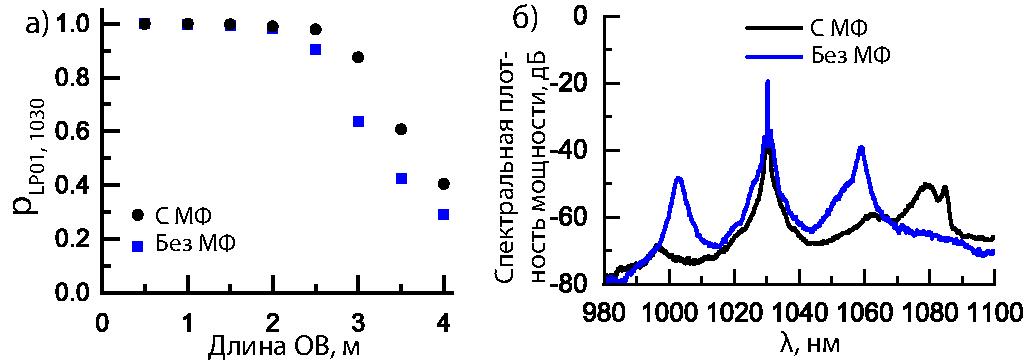
\includegraphics[width=0.99\linewidth]{Dissertation/images/imfwm/suppression_spectrum.pdf}
			\footnotesize{Зависимость доли оптической мощности $p_{\LPoi \text{, 1030}}$ моды $\LPoi$ в диапазоне длин волн $1030.0\pm0.5~\text{нм}$ на выходе ОВ доставки от его длины (a) и выходные спектры для длины ОВ доставки $L=4~\text{м}$ (б) с применением и без применения МФ на его входе}
		\end{column}
	\end{columns}	
	
\end{frame}

\begin{frame}
	\frametitle{Ответы на замечания Макарова~Д.Н.}
	\textbf{Замечание 2 из 3}: В главе 4 при оценке влияния непостоянства коэффициента теплоотдачи предполагается, что при нагреве и охлаждении коэффициент теплоотдачи принимает различные, но постоянные значения. Насколько это допущение соответствует кинетике конвективного теплообмена в условиях реального эксперимента?
	
	\hfill
	
	\textbf{Ответ:} Представляется возможным указать следующие факторы:
	
	\begin{itemize}
		\item \textbf{Развитие конвективных потоков:} нагрев начинается из состояния покоя,  охлаждение — с уже сформировавшегося конвективного течения.
		\item \textbf{Влияние конечной теплопроводности}: при нагреве температурное поле более неоднородно, чем при остывании, то есть одинаковым средним температурам соответствуют разные температуры границы кристалла, что эффективно влияет на определяемый в эксперименте $h$.
		\item \fixme{что-то ещё?}
	\end{itemize}
	
	
	
\end{frame}


\begin{frame}
	\frametitle{Ответы на замечания Макарова~Д.Н.}
	\textbf{Замечание 3 из 3}: В работе не выдержано единообразие в использовании сокращений. В частности, понятие «нелинейно-оптический» встречается как в сокращённой форме («н-о»), например, на стр. 4, 5, так и в полной, например, на стр. 56, 78.
	
	\hfill
	
	\textbf{Ответ}: Замечание принято, будет учтено в дальнейшей работе. 
	
	
\end{frame}